\section{Influence of other parameters}
\label{influence}

On this part we will look at how the parameter like the distance between the primary and the sun affect the thermal model or how the thermal inertia is also impacting the model.
We have worked on the case of the satellite called \textit{Juventas}.

It show us the graph you can see below : 

\begin{center}
	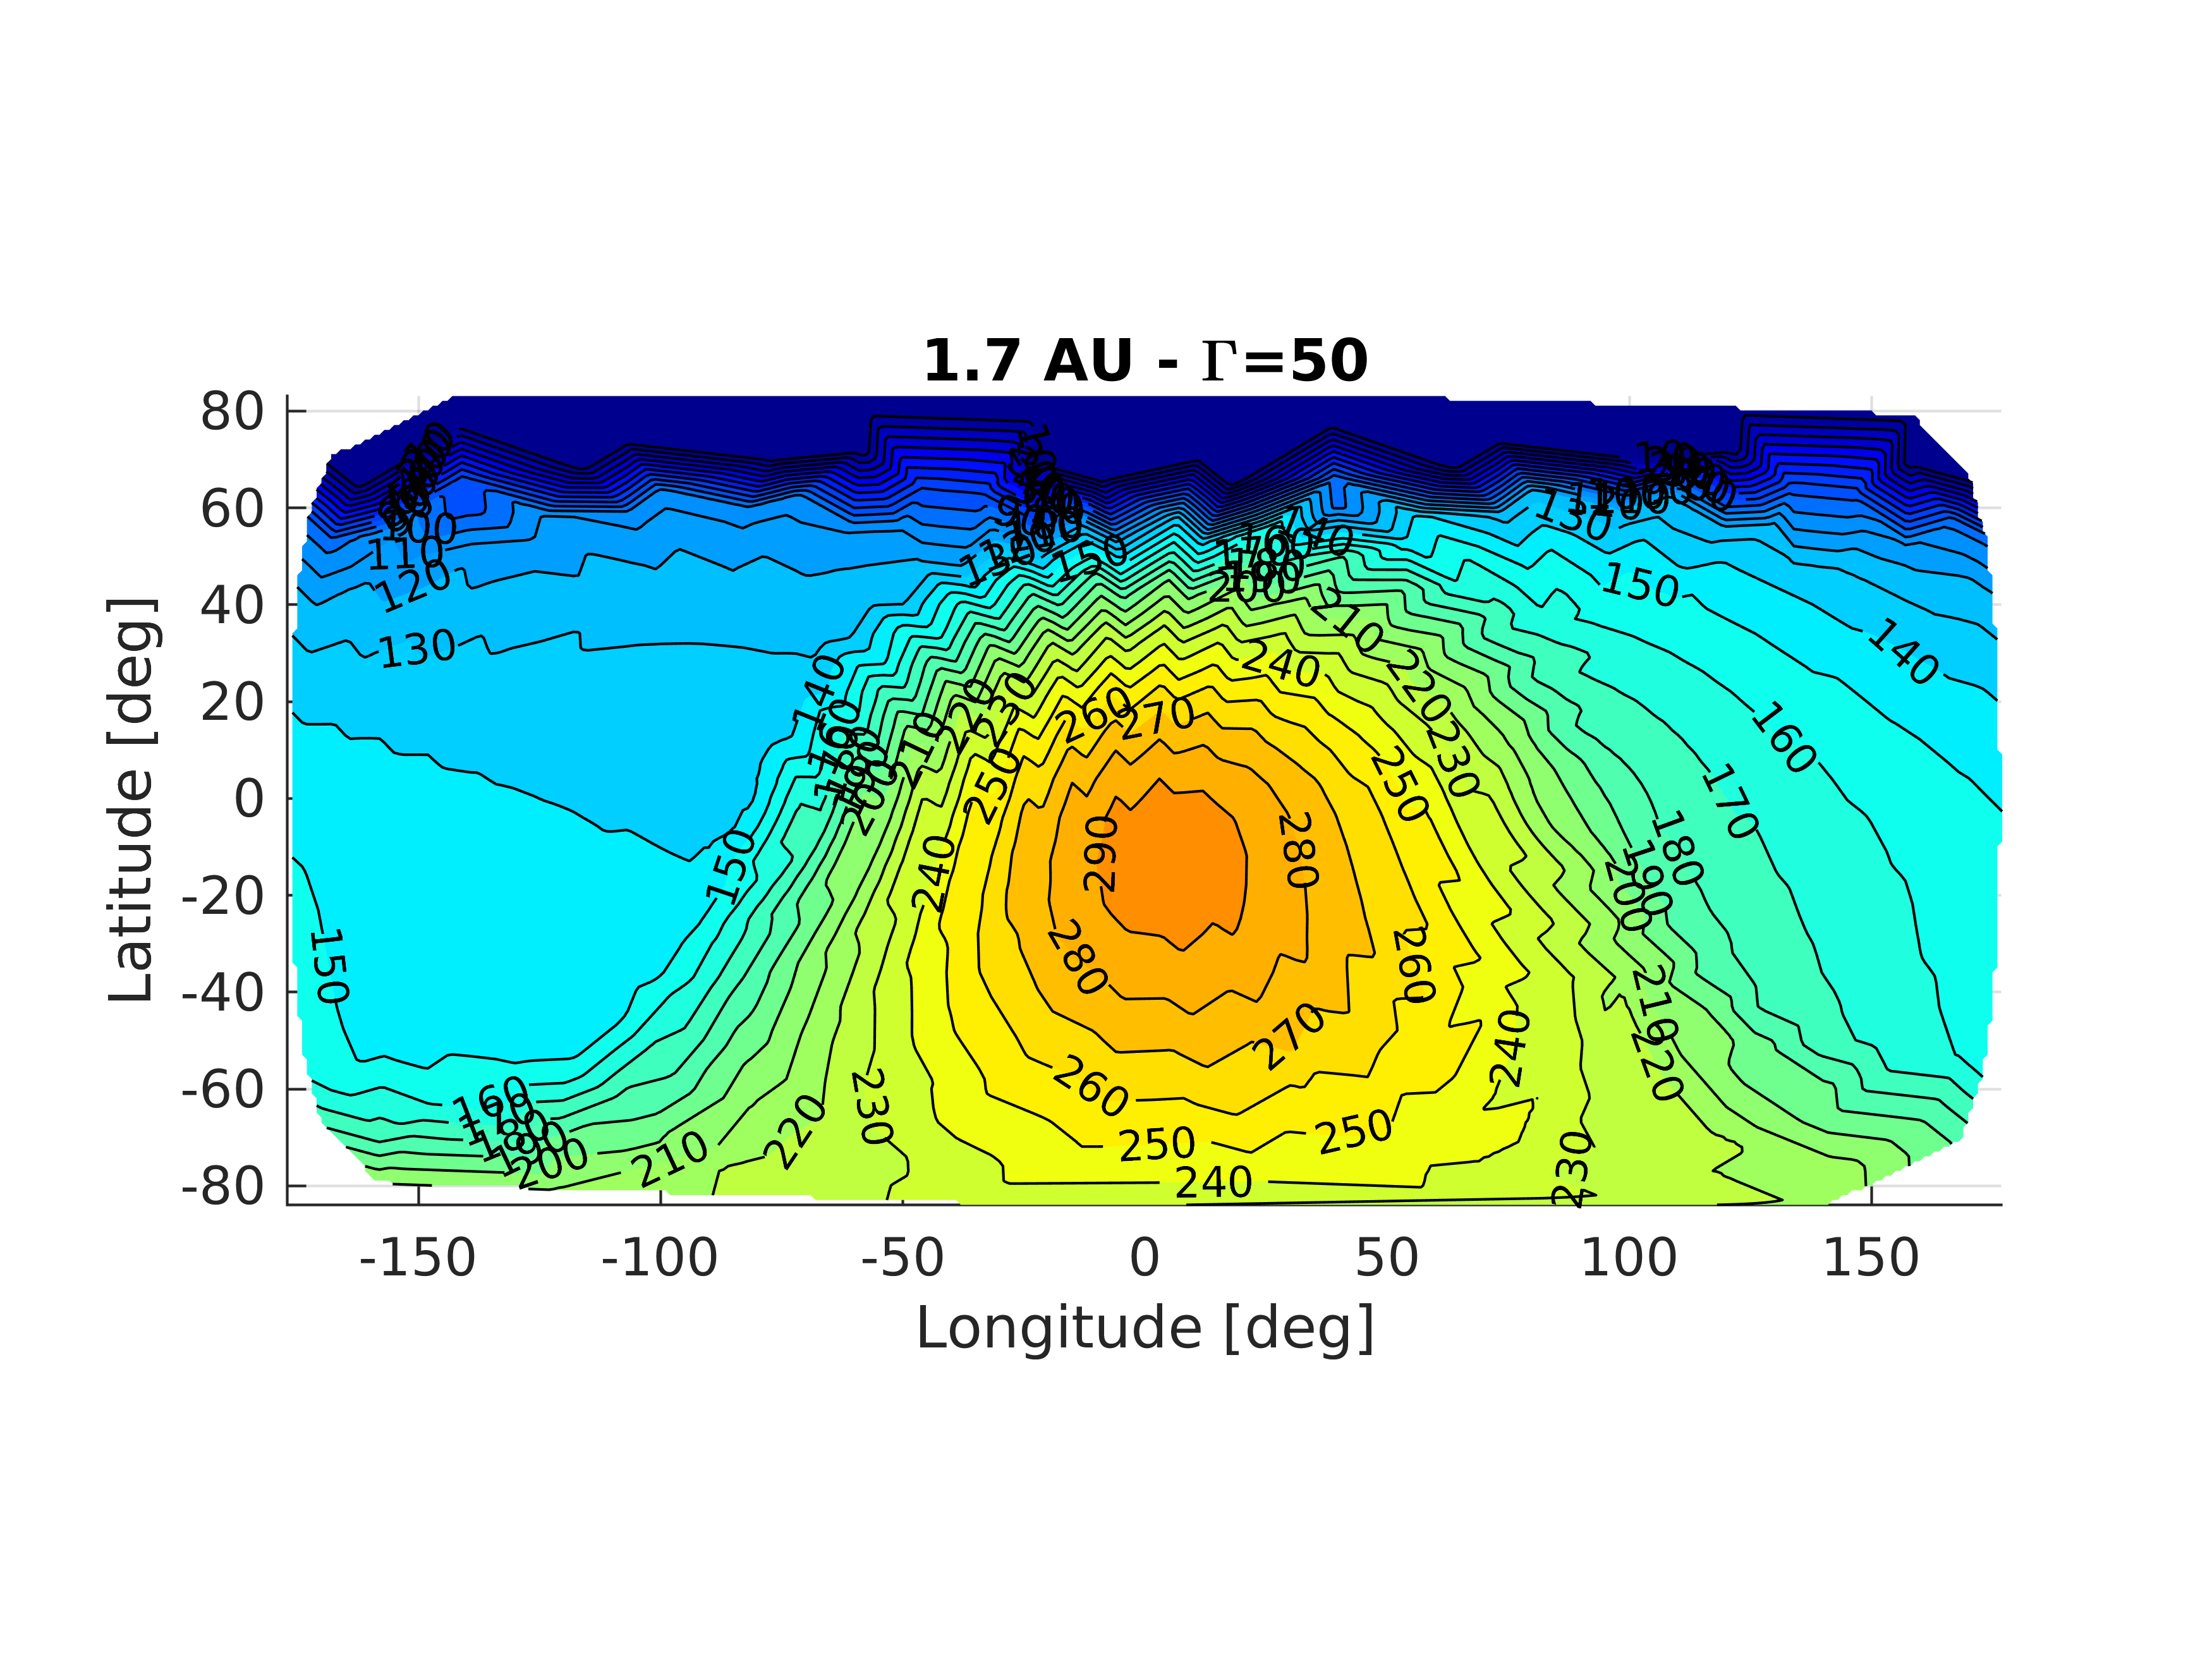
\includegraphics[scale=1]{rsc/juventas_d1.7_g50.png}
	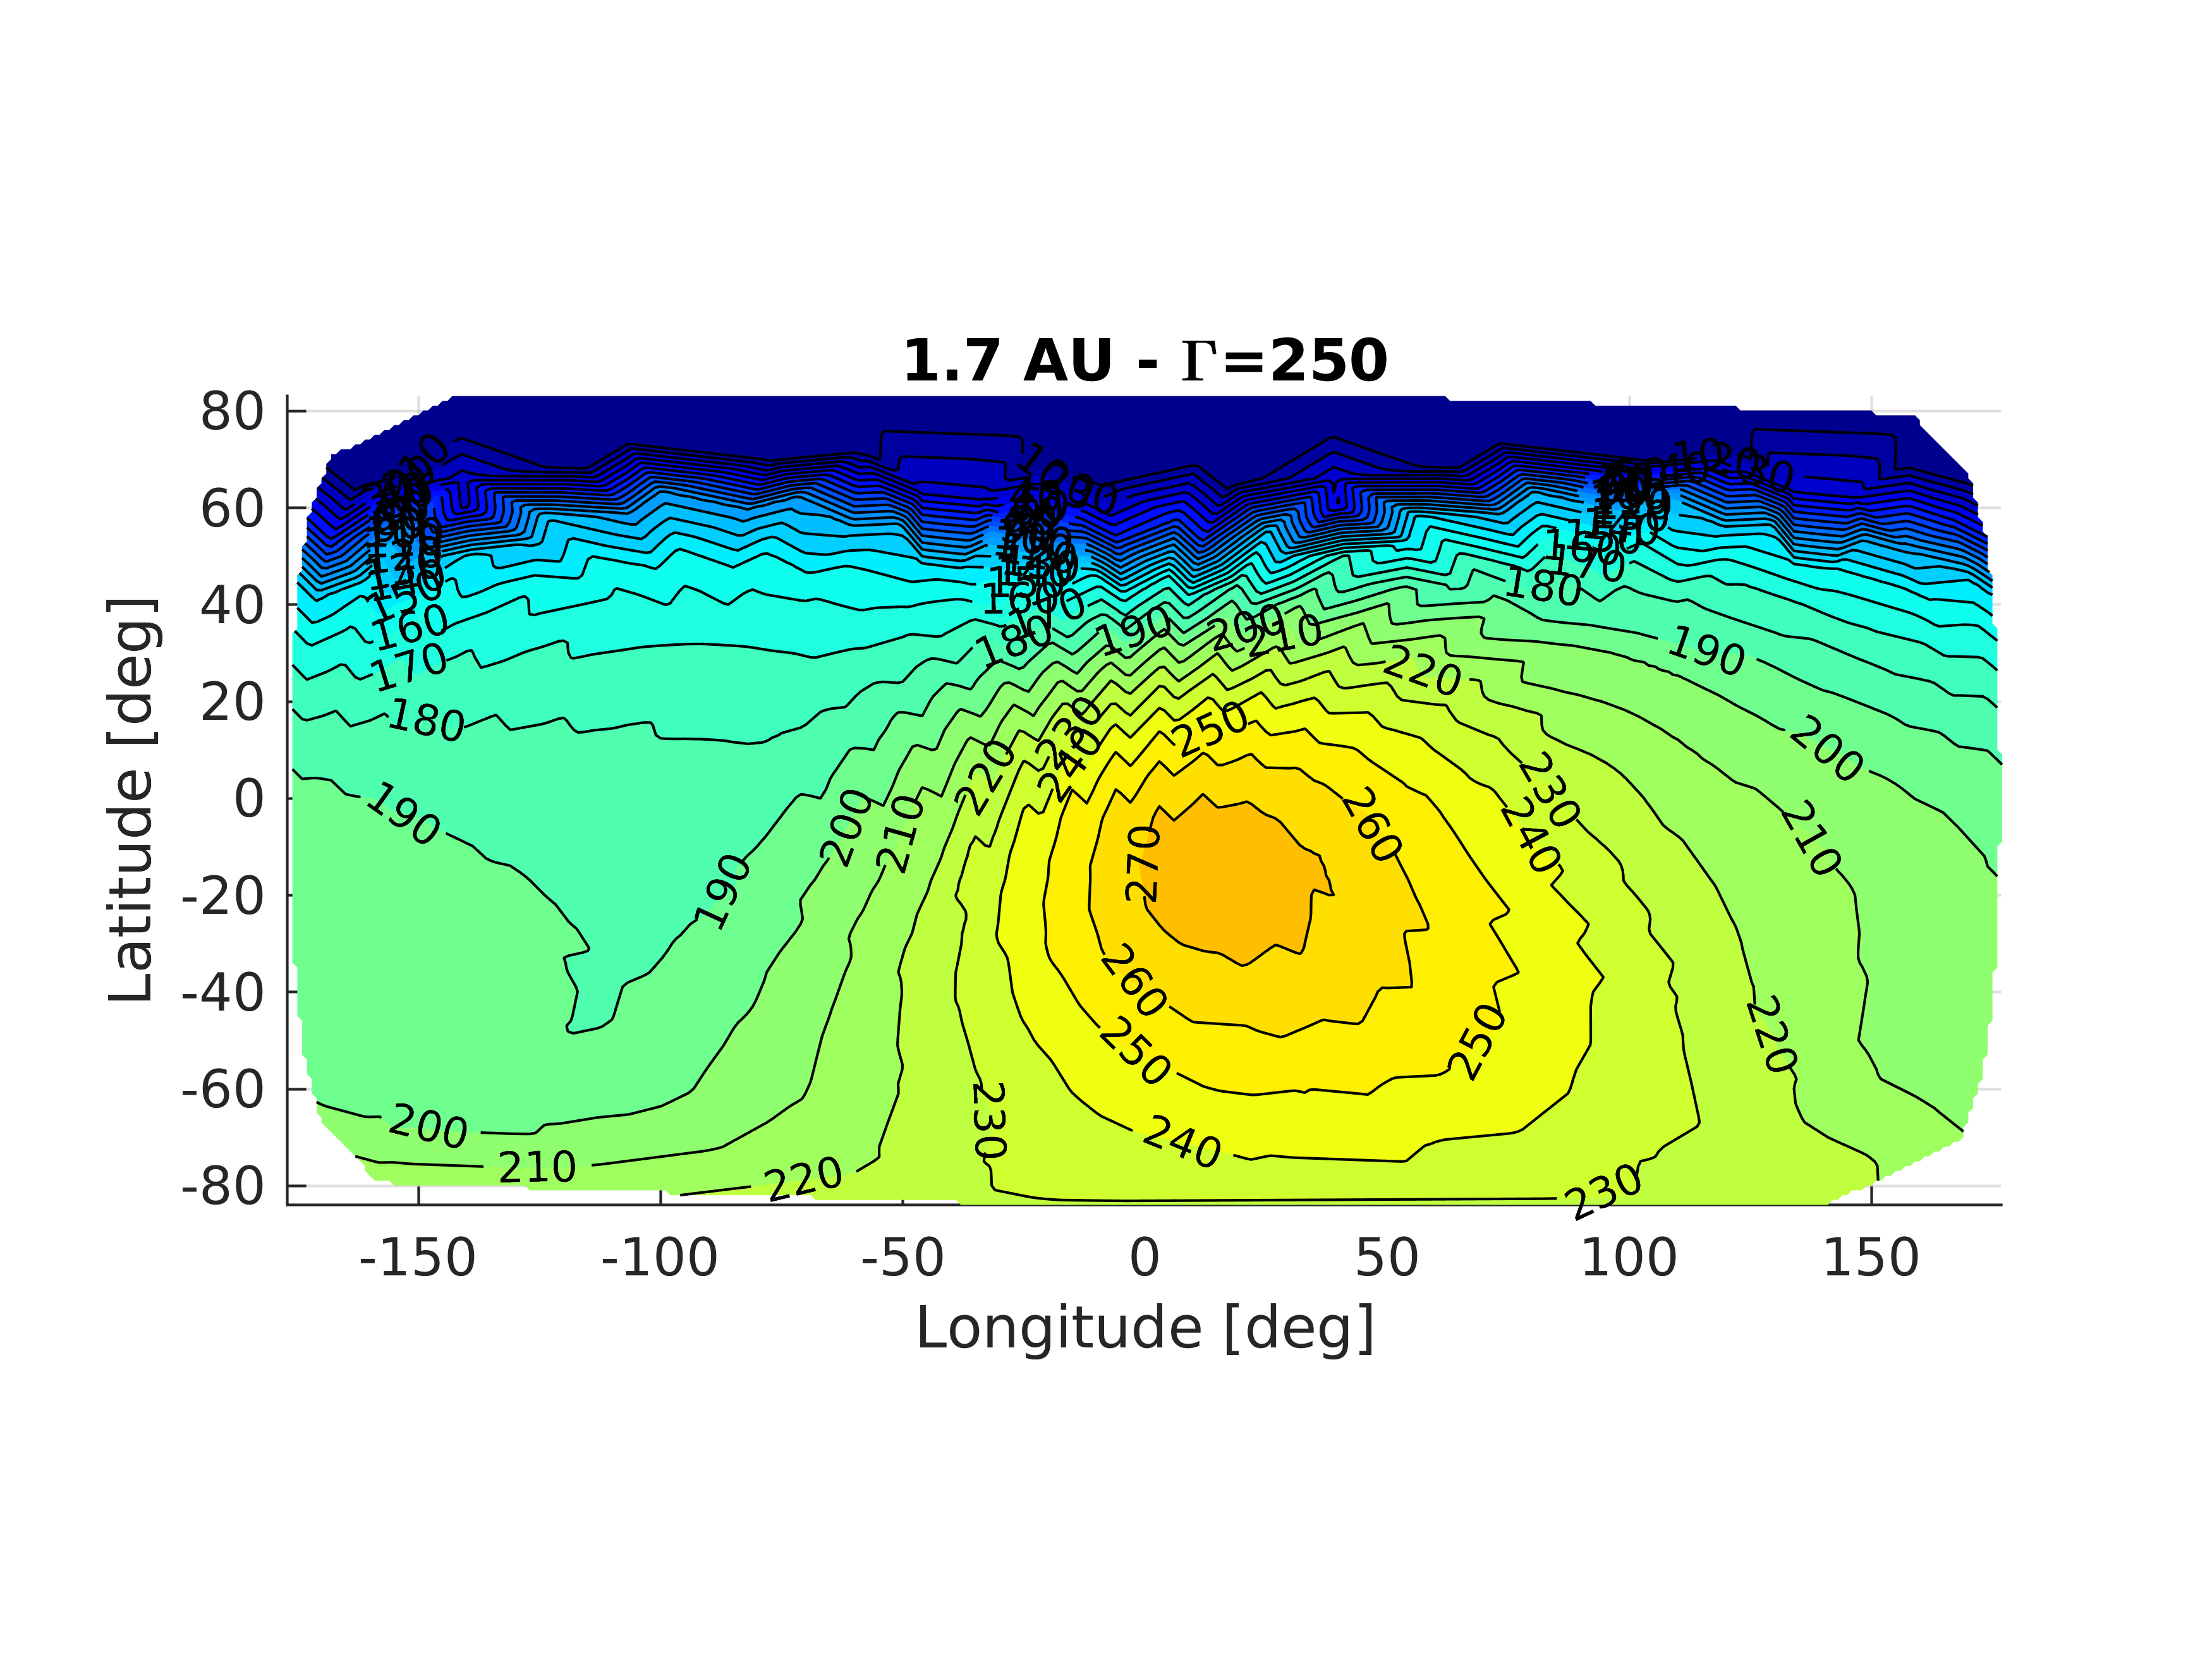
\includegraphics[scale=1]{rsc/juventas_d1.7_g250.png}
	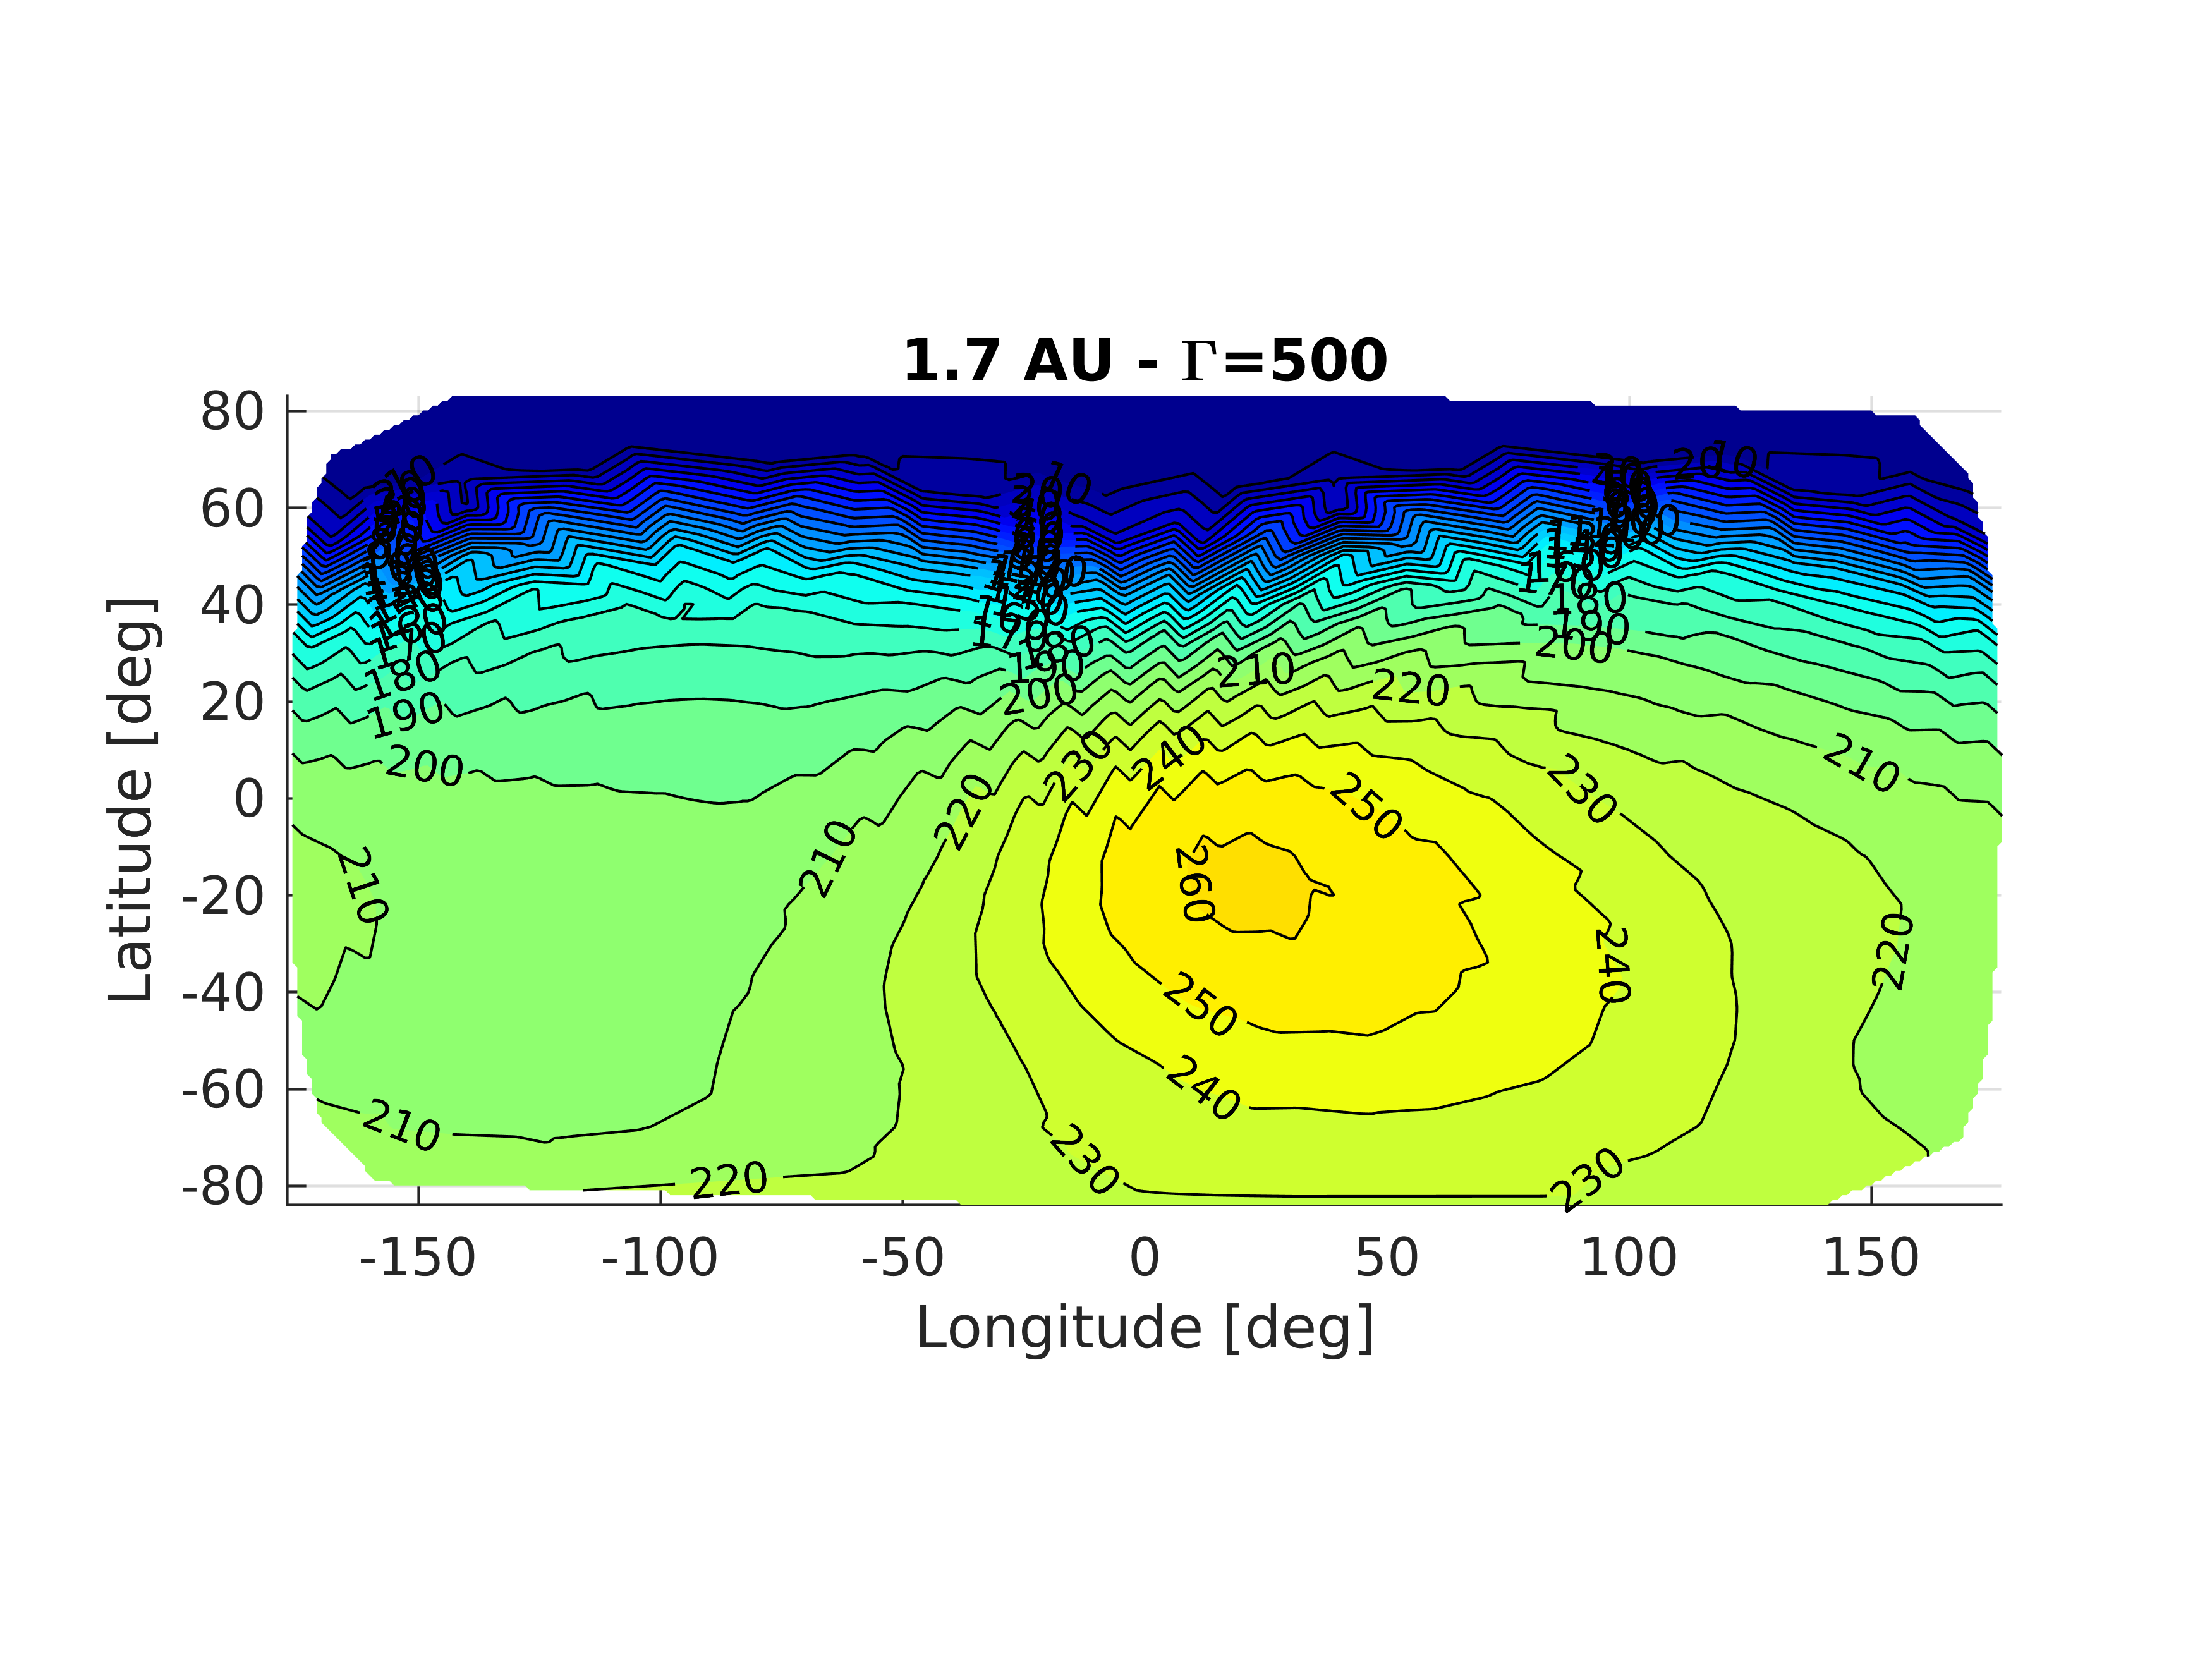
\includegraphics[scale=1]{rsc/juventas_d1.7_g500.png}
	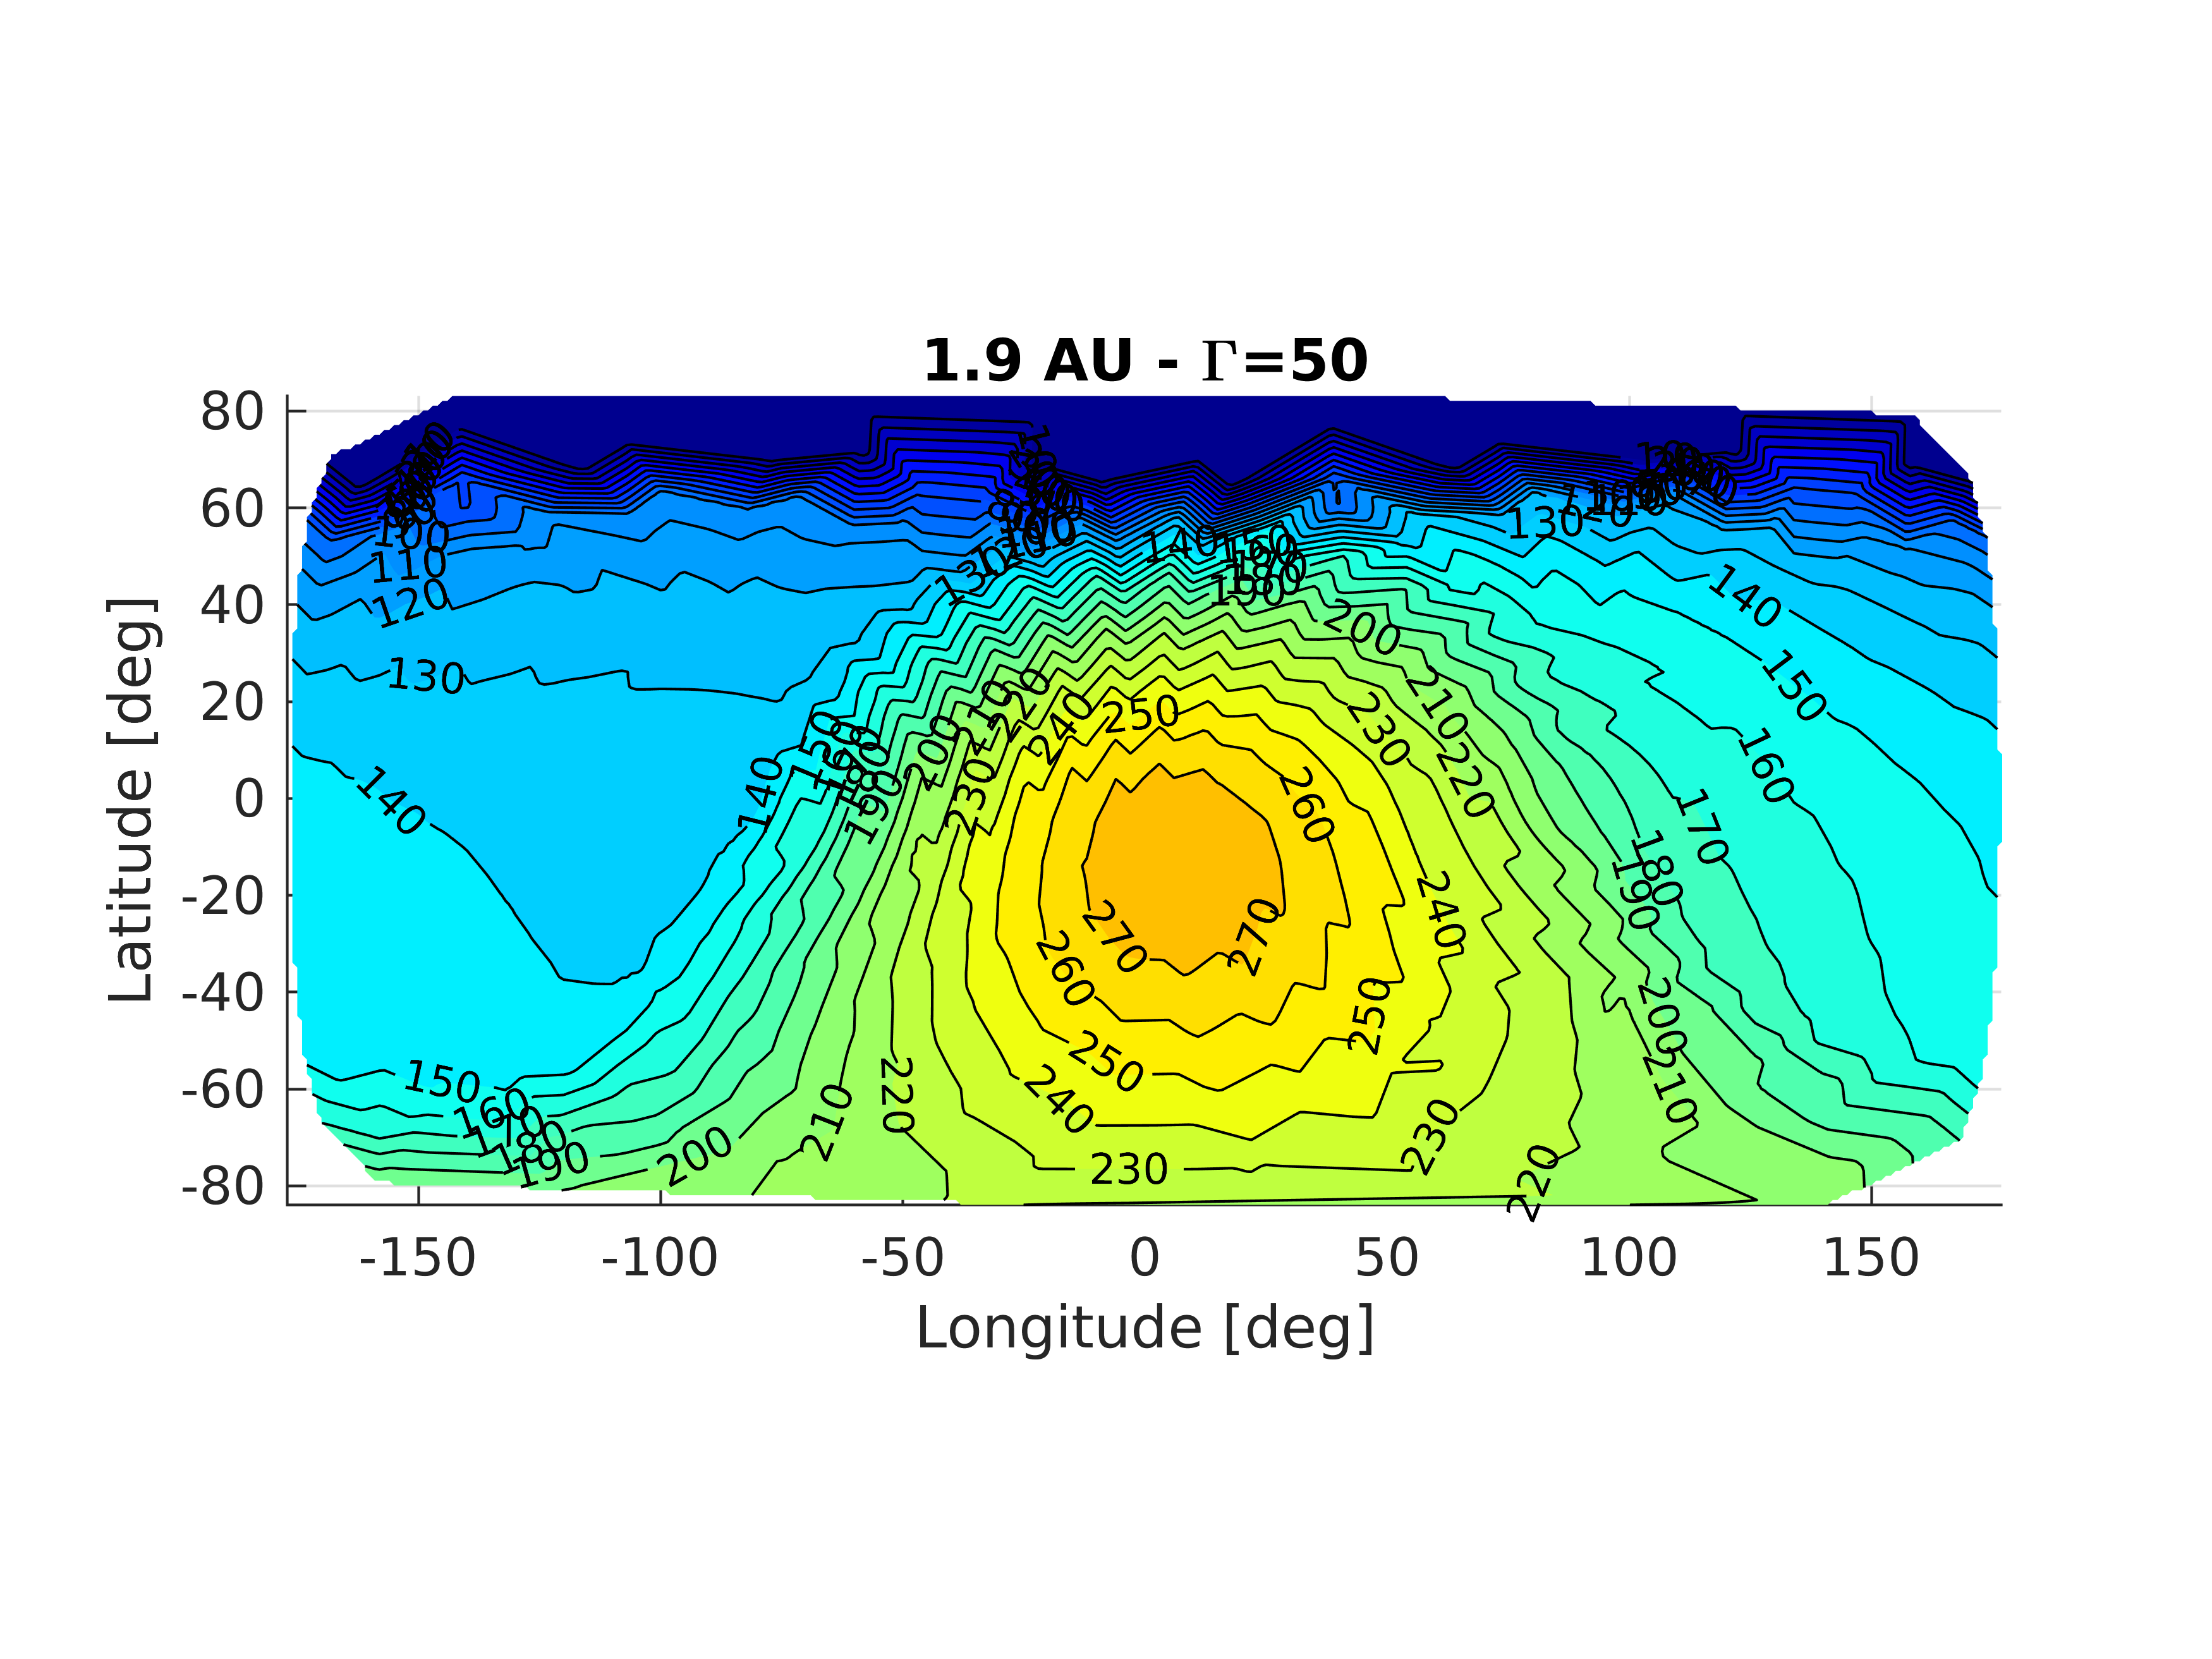
\includegraphics[scale=1]{rsc/juventas_d1.9_g50.png}
	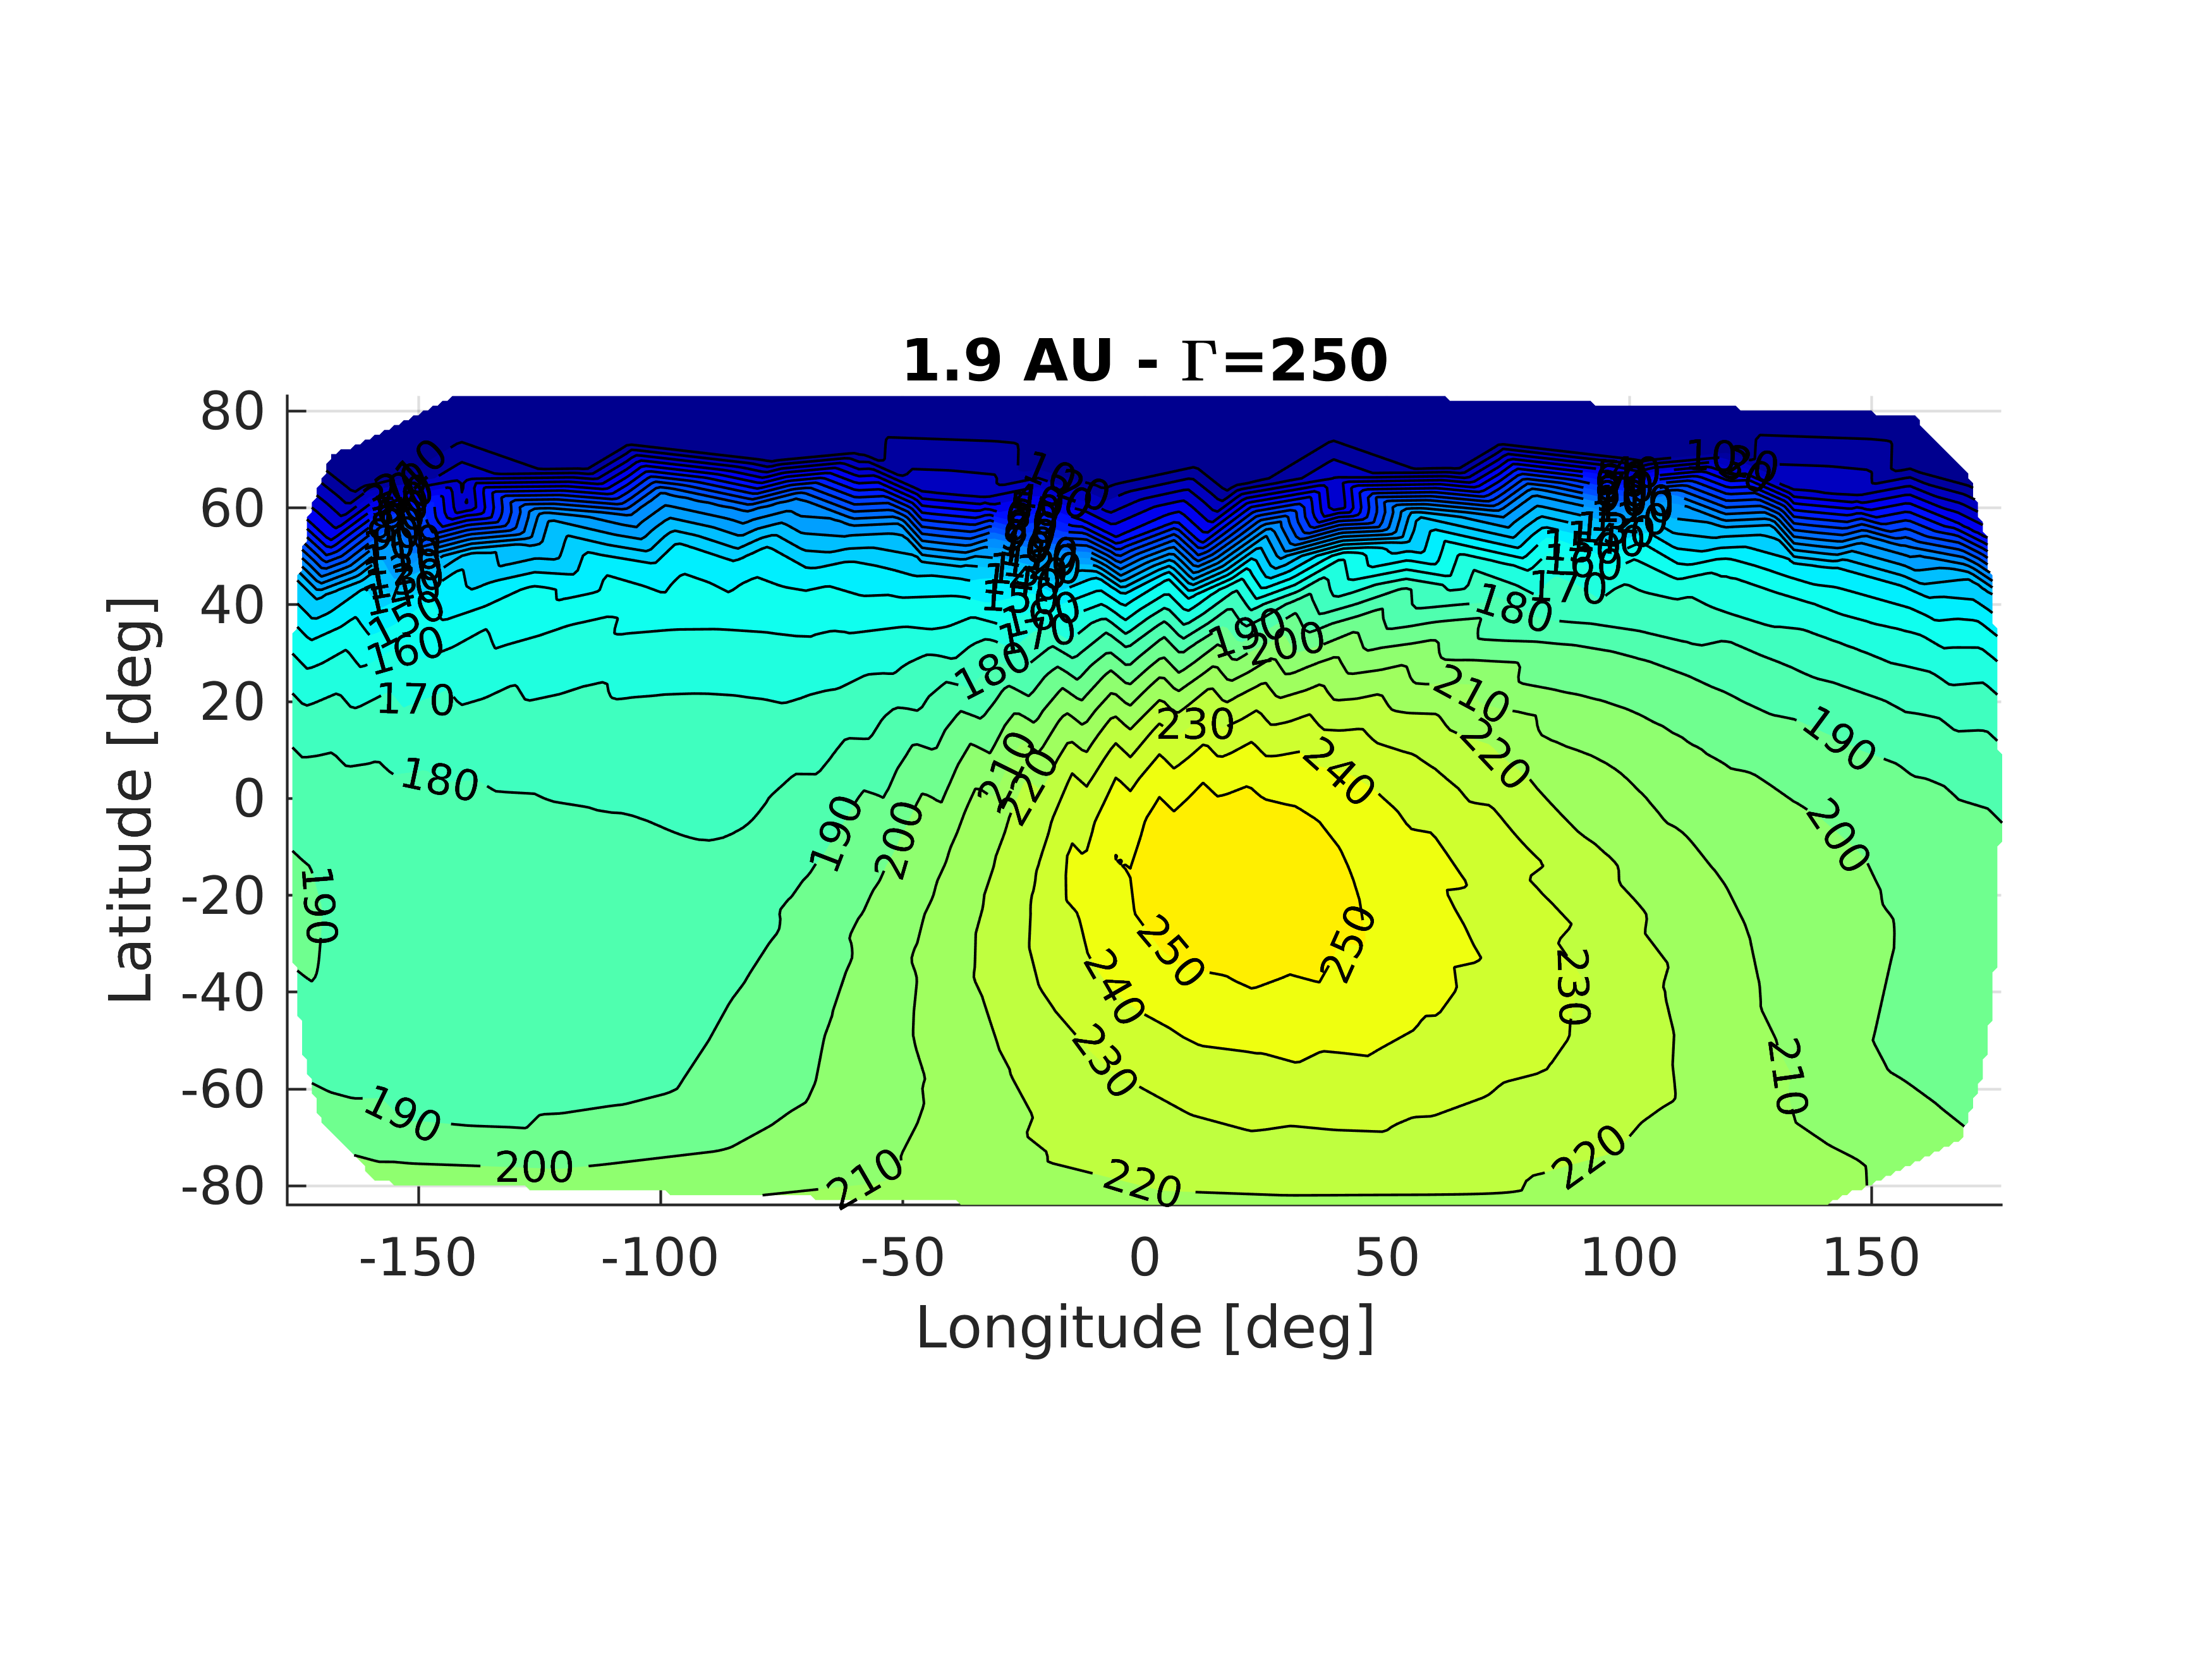
\includegraphics[scale=1]{rsc/juventas_d1.9_g250.png}
	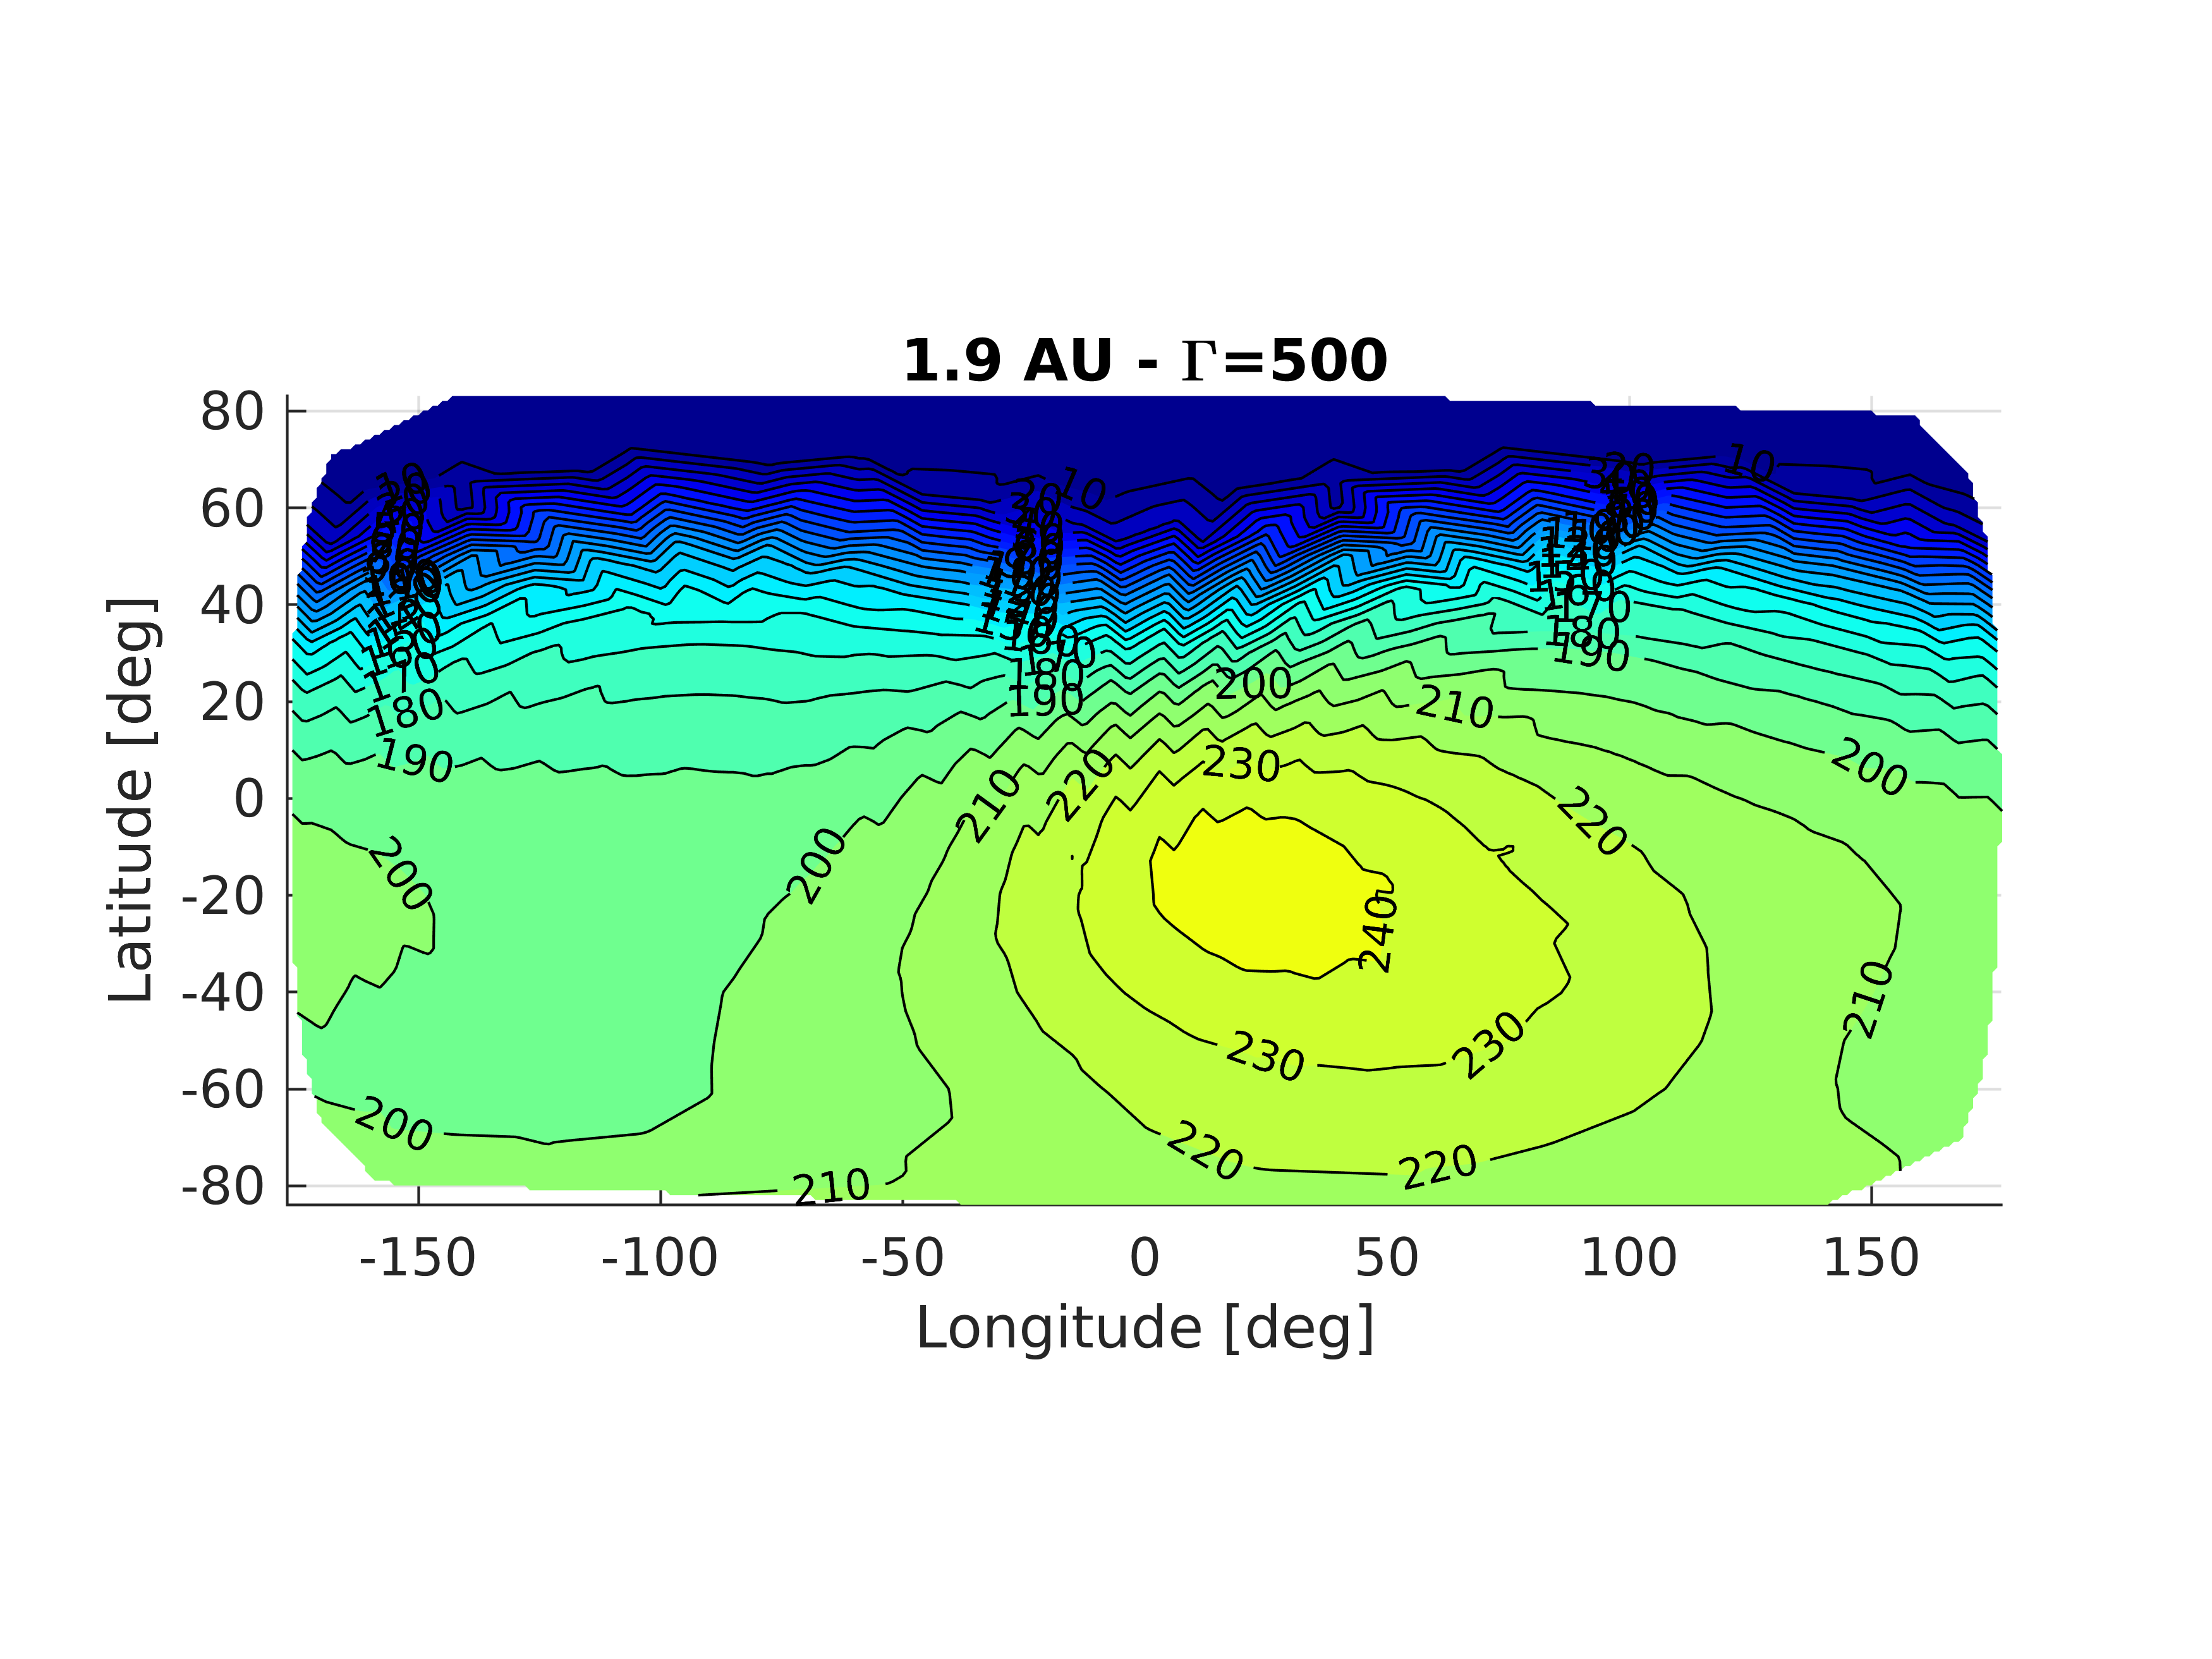
\includegraphics[scale=1]{rsc/juventas_d1.9_g500.png}
	\captionof{figure}{The different value of \Gamma and §r_{primary, sun}§}
\end{center}

We obtain this different thermal model, the distance is impacting on the direct flux, which contribute to increase of decrease the temperature of the object. As we can see the different distance does not modify a lot the temperature but we only have taken $0.2$ au difference, so we can imagine that with a bigger distance the value of the temperature will decrease a lot.\\[10pt]
Now we will look a the \Gamma, the higher the thermal inertia is, the less it is impacted from temperature changes and the slowest it conducts the heat.